\documentclass[main.tex]{subfiles}

\begin{document}

\section{Presentation of the Context}\label{sec:presentation-of-the-context}

Tor and IPFS are born and developed to face challenges related to privacy, security and decentralization of information on the internet.\\
They also allow access to online content that could be censored or blocked in certain regions.\\
Websites hosted on TOR are often more difficult to censor or block, thus helping to ensure freedom of information.\\
Similar speech for IPFS where people can publish content without having to rely on a centralized server. This way, content remains accessible even if some nodes in the network are disconnected or censored.


\subsection{Aim of the Dapp}
Accessing such data can be inconvenient as resource addresses are represented with poorly manageable hash keys.\\
In this regard, Geth Domains is born, a decentralized application created with the aim of encouraging a platform to associate complex TOR and IPFS addresses to more "friendly" .geth addresses.\\
This helps create a more accessible and user-friendly ecosystem on the Ethereum blockchain.\\
\newline
We decided to rely on a decentralised system as it offers several advantages including immutability and transparency of data, the absence of an intermediary and resistance to censorship.

\subsection{Immutability}
The data on a blockchain is immutable once it has been confirmed. This means that once a domain name is registered on GethDomains, it is difficult to change or delete it without the network’s consent. This contributes to the stability and security of the system.\\
The only one able to perform operations on the domain is the possessor.

\subsection{Censorship}
No single central authority has complete control over the domain name registry.\\
This makes it more difficult for government authorities or other entities to censor, block or confiscate specific domain names.

\subsection{No Third Parties}
It is not necessary to rely on central intermediaries such as registers of traditional domains.\\
This reduces the risk of manipulation, censorship or other interference by centralized third parties.\\
The lack of an intermediary also leads to cost savings and greater efficiency as well as an increase in ownership control by the user as they are not dependent on anyone.

\subsection{Permissionless Blockchain}
We decided to use the blockchain as there is the need to save all transactions linked to a domain in a clear and transparent way.\\
In this way anyone who makes purchases can register the new ownership by writing on the blockchain.\\
The blockchain, in this context, plays the role of impartial intermediary within this ecosystem without knowing a priori who will use it.\\

\begin{center}
  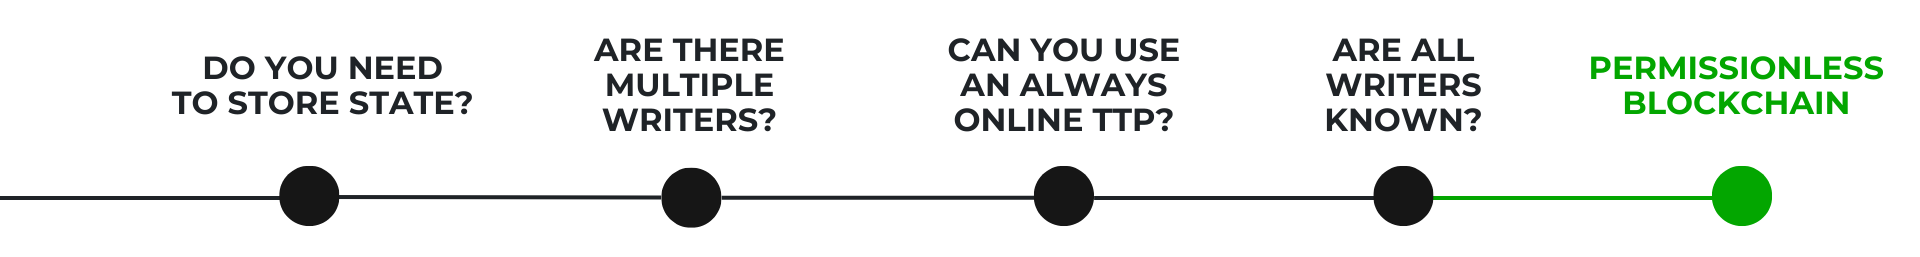
\includegraphics[height=2cm]{figures/PermBlock.png}
\end{center}

\subsection{Use cases}
Our platform will allow you to register your IPFS or TOR domain by associating an address with it. Geth, put it on sale if you do not want to have more possession and therefore offer a marketplace to buy domains to users.\\\\
The domains will be registered on the ethereum blockchain via NFT and all operations carried out thanks to the native currency of the Dapp: GETH Token.\\
In addition, when a user sells his domain you will see a system of royalties that will allow him to earn a lifetime on each future sale and subsequent transfer of ownership.\\\\
All the operations mentioned here will be seen in the next section and in particular we will go into detail of the two smart-contracts, one for the token and one for the Dapp, which allow the existence of this ecosystem and the absence of intermediaries.







\end{document}